You plug in your shiny, new keyboard, tune your satellite radio to the Greatest Hits of the 1920s, and settle in to solving a more interesting problem.

To protect against corporate espionage, you are responsible for writing code for a challenge-and-response system.
Anybody can challenge anyone else in the Pleistocene Petting Zoo's non-public areas by providing the name of a book and a word contained within the book, and the person being challenged must respond with another word from that book, based on certain rules:
\begin{itemize}
    \item All of the book's words are sorted alphabetically without regard to capitalization (for example, ``hello'' occurs after ``Hear'' and before ``HELP'')
    \item The challenge word occurs \textit{occurrences} times in the book
    \item If $occurrences$ is an odd number then the response word is the word $occurrences$ places \textbf{after} the challenge word in the alphabetized list;
    if the challenge word is less than $occurrences$ places from the end of the list then ``wrap around'' to the start of the list and resume counting
    \item If $occurrences$ is an even number then the response word is the word is ${2 \times occurrences - 1}$ places \textbf{after} the challenge word in the alphabetized list;
    if the challenge word is less than ${2 \times occurrences - 1}$ places from the end of the list then ``wrap around'' to the start of the list and resume counting
\end{itemize}

Here is a simple example.
Suppose the words in the specified book are:

\begin{center}
    \begin{tabular}{cc}
        \textit{word} & \textit{occurrences} \\ \hline
        apple       & 7 \\
        banana      & 4 \\
        carrot      & 15 \\
        date        & 3 \\
        eggplant    & 2 \\
        fig         & 6 \\
        granola     & 9 \\
        horseradish & 9 \\
        ice         & 6 \\
        jelly       & 3 \\
        kale        & 1 \\
        lemon       & 2 \\
        mango       & 8 \\
        naan        & 7 \\
        orange      & 5 \\
        pineapple   & 1 \\
        quinoa      & 11 \\
        raisin      & 4 \\
        spaghetti   & 10 \\
        tomato      & 12 \\
    \end{tabular}
\end{center}
If the challenge word is ``horseradish'' then because horseradish occurs 9 times in the book, the response word is ``quinoa,'' which is 9 places in the list after ``horseradish.''
If the challenge word is ``eggplant'' then the response is ``horseradish,'' which is 3 places ($2 \times 2 - 1 = 3$) later in the list than ``eggplant.''
If the challenge word is ``quinoa'' then the response word is ``horseradish,'' because the response word should be 11 places after ``quinoa,'' but the end of the list is 3 places later;
``horseradish'' is in position 8 in the list ($11 - 3 = 8$).
(\textit{Note:} ``horseradish'' and ``quinoa'' being each other's response words is coincidental.
Unusual things happen with short lists of words that do not generalize to longer lists.)

You break the problem down into four sub-problems:

\begin{enumerate}
    \item Designing the Data Structure and Its Algorithms
    \item Alphabetizing Words
    \item Inserting Words
    \item Responding to a Challenge
\end{enumerate}

\subsection*{The Books}

Four small ``books'' are included with the starter code:

\begin{itemize}
    \item ``Animals'' (sorted, 7 words)
    \item ``Plants'' (unsorted, 7 words)
    \item ``Cars'' (sorted, 74 words)
    \item ``Food'' (unsorted, 125 words)
\end{itemize}

Two real books have also been reduced to one word per line:\footnote{The text for these books was obtained from \href{https://www.gutenberg.org/}{Project Gutenberg}.
In accordance with Paragraph~1.C of the \href{https://www.gutenberg.org/policy/license}{Project Gutenberg License}, all references to Project Gutenberg have been removed from the ``derived works'' that we are distributing.
(Removing the references to Project Gutenberg was also necessary to ensure that \textit{only} the words from the books are used for the challenge-and-response system.)}

\begin{itemize}
    \item Mary Shelly's \textit{Frankenstein; Or, The Modern Prometheus} (filename ``Frankenstein'') \url{https://www.gutenberg.org/ebooks/84} (sorted, 74,363 words)
    \item Arthur Conan Doyle's \textit{The Lost World} (filename ``TheLostWorld'')
    \url{https://www.gutenberg.org/ebooks/139} (unsorted, 77,268 words)
\end{itemize}

The very small files of 7 words can be useful for debugging, and the moderate-sized files of 74--125 words should give you confidence in the correctness of your solution.
The real books of more than 74,000 words will be useful to reveal whether you have any memory leaks in your code.
The files marked as \textit{sorted} have all of their words already in alphabetically sorted order, ignoring capitalization;
the files marked as \textit{unsorted} do not have their words sorted (the words in ``Plants'' and ``Food'' are in a randomly-selected order;
the words in ``TheLostWorld'' appear in the order that they appear in the original \textit{The Lost World}).

Each book file, ``\textit{file}'', has a corresponding ``\textit{file}-table.md'' that contains a Markdown-formatted table of the challenge words, the number of occurrences for each challenge word, and the corresponding response word.
You may use these files to confirm the correctness of your solution.

Throughout the assignment, we note that if building the list takes more than a few seconds, there is a bug in your code;
for context, we can build the list for \textit{Frankenstein} in 1--2 seconds and the list for \textit{The Lost World} in 1.5--3 seconds.
We can locate a word (or determine the absence of a word) in the \textit{Frankenstein} list in under 0.5ms and in the \textit{The Lost World} list in under 0.9ms.
Your code may take longer, but it should not take much longer.

You will earn most of the credit for this lab if your code works for pre-sorted files of up to 200 words.
The remaining credit is for making your code work with unsorted files and, when using files of up to 80,000 words, your code can generate a list and find a word in fewer than 20 seconds.

\subsection{Differences and Similarities between Java and C that are Relevant to this Assignment}

In some regards, Java keeps things simple: every variable is a reference, except when it isn't.
In other regards, C keeps things simple: you always know whether the variable you're using is a value or a pointer.

\subsubsection{Comparing Strings}

You probably learned that when comparing Java Strings, using the equality operator \lstinline{==} is error-prone.
When comparing two String literals (or variables assigned to String literals), the equality operator usually acts as a naive programmer would expect:
\lstinline{"abc" == "abc"} evaluates to \lstinline{true}.
When one or both of the Strings are generated at runtime, such as from user input, then the equality operator rarely evaluates to \lstinline{true}:
\lstinline{userInput == "abc"} will evaluate to \lstinline{false} even when the user entered ``abc''.

The reason for this is that when comparing objects (other than boxed types), Java's comparators compare the objects' references;
that is, Java comparators compare the objects' memory addresses.
Using the \lstinline{==} operator to compare Strings evaluates to \lstinline{true} only when the two Strings occupy the same address;
that is, they are both literally the same String object.
This is why you were taught to use Java's \function{String.equals()} method to compare strings.

Comparing C strings' variables has the same pitfall:
because the string variables are pointers to the first character in their respective strings, using arithmetic comparators will compare the strings' addresses.
If you want to compare two C strings, you would use the \function{strcmp()}\footnote{See footnote~\ref{note:stringFunctions}.} function.
The wrinkle is that \function{strcmp()} returns \lstinline{0} (\textit{i.e.}, \lstinline{false}) when the two strings are equal;
you will often see the idiom \lstinline{if (!strcmp(string1, string2)) {}.

The \function{strcmp(string1, string2)} function actually performs a lexicographic comparison of the strings, returning a negative value if \lstinline{string1} occurs alphabetically earlier than \lstinline{string2}, zero if every character in the two strings match, and a positive value if \lstinline{string1} occurs alphabetically later than \lstinline{string2}.
In this regard, C's \function{strcmp()} function is more like Java's \function{String.compareTo()} method than \function{String.equals()}.

\subsubsection{Copying Strings}

Because Java Strings are immutable objects, you can safely copy a string by simply copying its reference (this is called \textit{aliasing}).
You can safely write the statement \lstinline{string1 = string2;} without worrying about changes to \lstinline{string2} causing changes in \lstinline{string1}
(if you were to make changes to \lstinline{string2}, it would result in a new String object being assigned to the \lstinline{string2} variable).

For mutable objects, creating an alias (that is, copying the reference) results in the situation that changes made through one variable are visible through the other variable.
For example, if you have the statements \lstinline{list1 = list2; list2.add(foo);} then \\ \lstinline{list1.size() == list2.size() && list1.contains(foo)} will evaluate to \lstinline{true}.
If the object's class implements the \lstinline{Cloneable} interface then you can make a copy of an object without aliasing it.
If you have the statements \lstinline{list1 = list2.clone(); list2.add(foo);} then \lstinline{list1.size() == list2.size()} will evaluate to \lstinline{false}.

In general, C strings are mutable.\footnote{
    The exceptions are string literals, which are immutable, and strings declared as a pointer to a constant, which if treated as mutable will result in undefined behavior.
}
This means that you generally don't want to create an alias.\footnote{
    Sometimes you can't create an alias.
    If the left-hand-side of an assignment is a constant pointer or is effectively a constant pointer -- such as an array inside a struct -- then it cannot be re-assigned.
}
Instead, use the \function{strcpy(destination, source)} or \function{strncpy(destination, source, n)}\footnote{See footnote~\ref{note:stringFunctions}.} function to copy the \lstinline{source} string into the memory pointed to by \lstinline{destination}.
The \function{strcpy()} function will continue copying until encountering the terminating \lstinline{NUL} in the \lstinline{source} string -- this is very slightly faster (not enough that you'd notice) but is safe only if you can prove that \lstinline{destination} has enough memory allocated for the string.
The \function{strncpy()} function will copy until encountering the terminating \lstinline{NUL} or until it has copied $n-1$ characters (after which it will append a terminating \lstinline{NUL}) -- this is safer because you can ensure that the string copied to \lstinline{destination} will fit within the space allocated for it.

\subsubsection{Allocating and Deallocating Memory}

As we'll note in Section~\ref{subsubsec:equivalentJava}, Java's \lstinline{new} keyword allocates space for the new object, inferring the amount of space needed based on the class's definition.
In C, you use the \function{malloc()} function to allocate space\footnote{
    There are a small handful of alternate functions, each with their own use cases, but \function{malloc()} is most-suitable for this lab.
}, and you must be explicit about how much space you need.
An idiom is to combine \function{malloc()} with the \function{sizeof()} function, as you saw in PokerLab, and as you'll see near the start of Section~\ref{subsubsec:cImplementation}.

Java uses a \textit{garbage collector} to reclaim memory allocated for objects that are no longer in use.
The unpredictability of when garbage collection happens makes an automatic garbage collector unsuitable for many of C's uses.
For this reason (among others), the programmer is responsible for deallocating memory that is no longer needed.
This is done with the \function{free()} function.

While a variable will go out of scope at the end of the code block in which it was declared, memory allocated in that code block persists unless explicitly \function{free}d.
Once the last pointer pointing to that memory goes out of scope, you no longer have a way to \function{free} that memory, resulting in a \textit{memory leak}.
On the other hand, \function{free}ing memory while it is still being used by another pointer can result in undefined behavior.
This requires careful thought to make sure that you \function{free} all memory that you allocated, but only after it is safe to do so.

For many short-running programs, such as those you often write in school, you often can ignore the need to \function{free} allocated memory since all the program's memory will be reclaimed by the operating system when the program terminates.
A member of the C Standard Committee recently described this as having a maid that will clean up your mess.\footnote{
    \url{https://twitter.com/__phantomderp/status/1619322783162568705}, \\ \url{https://twitter.com/__phantomderp/status/1619323139665846273}
}

I advise you not to rely on that ``maid'' even for a ``short-running program,'' such as this one.
In an earlier version of this lab, there were a dozen or so students whose code, when tested against a 75,000-word file, would quickly consume all the server's physical memory.
As the first of these programs thrashed the virtual memory system, it prevented other services from working effectively, including the one that I had precautionarily introduced to kill a test after a couple of minutes.
It consumed enough resources that the system administrator couldn't log in to determine why the server had slowed to a crawl.
As I was already logged in, I was able to kill the process as the system administrator was preparing to disconnect the server from the power line.
The system administrator later commented about the resources it consumed, ``You ought never to see a `T' in the memory column'' (Figure~\ref{fig:tooMuchMemoryUsed}).

\begin{figure}
    \center
    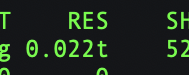
\includegraphics{too-much-memory-used}
    \caption{Screenshot showing a student's program consuming 0.022 terabytes of physical memory;
    the allocated virtual memory is not visible in the image.\label{fig:tooMuchMemoryUsed}}
\end{figure}

\subsubsection{Idioms for Defining and Initializing \texttt{Struct} Types}

In PokerLab, you worked with a struct that was defined by \lstinline{typedef} as a new type.
In this lab, you will work with a struct defined simply as a \lstinline{struct}, without a \lstinline{typedef}.
There are compelling arguments for and against both approaches in different use cases.
You should learn to be comfortable with both approaches.

In this lab, the function that initializes a node is also responsible for allocating space for that node.
In PokerLab, you saw the other idiom, in which the calling function is responsible for allocating space and passing the pointer to the initializer (this pointer is analogous to Java's implicit \lstinline{this} parameter).
The approach of having the caller allocate space seems to be more common, but both approaches are common enough to be aware of both.
(The third idiom is not to have a separate initializing function;
I discourage this approach.)

\subsection{Designing the Data Structure and Its Algorithms}

You decide that a circular linked list is the best data structure option for the challenge-and-response system.
You probably learned about linked lists in \cstwo; however, we will provide a refresher.

\subsubsection{Singly-Linked List} \label{subsubsec:singlylinkedlist}

A \textit{linked list} is a linear collection of data.
Like an array, each element (or \textit{node}) has a particular position in the list, and when you iterate over the list, you always access the elements in the same order every time (unless you change or re-order the elements).

In an array, the elements are contiguous in memory, and you can access a specific element by indexing the array (or, equivalently, performing pointer arithmetic).
In a linked list, however, the nodes can be in arbitrary locations in memory, and the nodes are connected by references (in C, pointers).
You can access a specific element only by following pointers from one node to the next until you reach the desired node.

The simplest linked list is a \textit{singly-linked list}.
A node consists of a \textit{payload} (the data that we care about) and a reference to the \textit{next} node;
see Figure~\ref{fig:singly-linked-list}.

\begin{figure}[h]
    \centering
    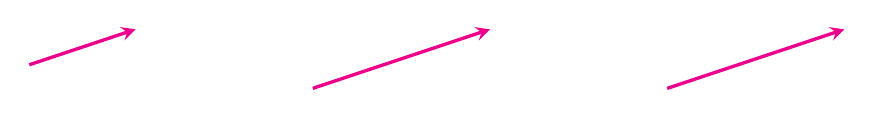
\begin{tikzpicture}[x=1.5mm, y=1.5mm]
        \draw[-stealth,very thick,magenta](-19,-3) -- (-10,0);
        \sllnode{0}{0}{0}
        \draw[-stealth,very thick,magenta](5,-5) -- (20,0);
        \sllnode{30}{0}{0}
        \draw[-stealth,very thick,magenta](35,-5) -- (50,0);
    \end{tikzpicture}
    \caption{Nodes in a singly-linked list consist of the payload data and a reference that points to the next node.}\label{fig:singly-linked-list}
\end{figure}

A linked list's greatest advantage over an array is that inserting and removing a node at an arbitrary location takes constant time, whereas inserting an element into an array (assuming there is sufficient memory allocated for the array) or removing an element from an array requires moving all the elements that follow the element's index.
Inserting a new node, $C$ between adjacent nodes $A$ and $B$ (where $B = A.next$) requires connecting $C.next$ to $B$ and re-assigning $A.next$ to $C$;
see Figure~\ref{fig:sll-insertion}.

\begin{figure}[h]
    \centering
    \begin{tikzpicture}[x=1.5mm, y=1.5mm]
        \draw[-stealth,very thick,magenta](-19,-3) -- (-10,0);
        \sllnode{0}{0}{0}
        \draw[-stealth,very thick,magenta](5,-5) -- (13,-5) -- (13,-12.5) -- (0,-12.5) -- (0,-25) -- (5,-25);
        \sllnode{15}{-25}{0}
        \draw[-stealth,very thick,magenta](20,-30) -- (30,-30) -- (30,-12.5) -- (17,-12.5) -- (17,0) -- (20,0);
        \sllnode{30}{0}{0}
        \draw[-stealth,very thick,magenta](35,-5) -- (50,0);
    \end{tikzpicture}
    \caption{Inserting a new node into a singly-linked list only requires assignments to the affected \textit{next} pointers.}\label{fig:sll-insertion}
\end{figure}

As with an array, you do need to maintain a variable that points to the list.
Conventionally, this is a reference to the \textit{head} of the list.
(Note that if a new node is inserted before the current head node, then the new node becomes the head of the list, and your \lstinline{head} variable would need to be updated.)
It is not uncommon to also maintain a reference to the \textit{tail} of the list.

\subsubsection{Circular Linked List} \label{subsubsec:circularlinkedlist}

A \textit{circular linked list} is a linked list in which the tail's \textit{next} field points to the head of the list.
In essence, a circular linked list has no head (because every node is some node's \textit{next}), and has no tail (because every node's \textit{next} is non-NULL);
see Figure~\ref{fig:circular-linked-list}.

\begin{figure}[h]
    \centering
    \begin{tikzpicture}[x=1.5mm, y=1.5mm]
        \sllnode{0}{30}{0}
        \draw[-stealth,very thick,magenta,rotate=0](5,25) -- (25.5,18.8);
        \sllnode{0}{30}{-72}
        \draw[-stealth,very thick,magenta,rotate=-72](5,25) -- (25.5,18.8);
        \sllnode{0}{30}{-144}
        \draw[-stealth,very thick,magenta,rotate=-144](5,25) -- (25.5,18.8);
        \sllnode{0}{30}{144}
        \draw[-stealth,very thick,magenta,rotate=144](5,25) -- (25.5,18.8);
        \sllnode{0}{30}{72}
        \draw[-stealth,very thick,magenta,rotate=72](5,25) -- (25.5,18.8);
    \end{tikzpicture}
    \caption{A circular linked list does not have a well-defined head and tail.}\label{fig:circular-linked-list}
\end{figure}

You still need to maintain a variable that points to \textit{some} node in the list.

\subsubsection{Equivalent Java Code} \label{subsubsec:equivalentJava}

In Java, you probably wouldn't implement your own linked list;
instead, you would use \lstinline{java.util.LinkedList}, which has been available since J2SE~1.2
(ignoring for the moment that Java's standard library doesn't have a circular linked list).
A list of hypothetical \lstinline{Payload} objects would be created with:
\begin{lstlisting}[numbers=none]
    List<Payload> payloads = new LinkedList<>;
\end{lstlisting}

C doesn't have a built-in linked list data type, so you will need to design one.
Let us consider what a custom linked list would look like in Java.

\begin{lstlisting}[mathescape=true]
public class Node {
    private final String word;          $\label{code:javaWord}$
    private int occurrences;            $\label{code:javaOccurrences}$
    private Node next;                  $\label{code:javaNext}$
    private Node previous;              $\label{code:javaPrevious}$

    public Node(String word) {$\lstsetnumber{\ldots}$
        ...$\lstresetnumber\setcounter{lstnumber}{11}$
    }

    public void insertAfter(Node existingNode) {$\lstsetnumber{\ldots}$
        ...$\lstresetnumber\setcounter{lstnumber}{22}$
    }
    ...$\lstresetnumber\setcounter{lstnumber}{98}$
}
\end{lstlisting}

Creating and inserting a new node would look something like this:

\begin{lstlisting}[firstnumber=200, mathescape=true]
    Node node = new Node("eggplant");   $\label{code:newNode}$
    Node otherNode = ... // code to determine where the new node goes
    node.insertAfter(otherNode);        $\label{code:javaInsertAfter}$
\end{lstlisting}

Recall that in Java, all variables except primitive types (such as \lstinline{occurrences} on line~\ref{code:javaOccurrences}) are references.
This means that the \lstinline{next} field on line~\ref{code:javaNext} is a reference to another Node, just as we described in Section~\ref{subsubsec:singlylinkedlist}.
The payload is the \lstinline{word} and how many \lstinline{occurrences} the word has, exactly what we need for the challenge-and-response system.

Recall also that in Java, the \lstinline{new} keyword allocates space for the new object, and the constructor call -- \lstinline{Node("eggplant")} -- initializes the object.

\subsubsection{C Implementation} \label{subsubsec:cImplementation}

In \textit{challenge-response.h}, you'll see a \lstinline{struct} with the same fields as our Java example:

\lstinputlisting[linerange=19-24, firstnumber=36]{../starter-code/challenge-response.h}

In \textit{challenge-response.c}, you'll also see the \function{create_node()} function:

\lstinputlisting[linerange=23-29, firstnumber=23]{../starter-code/challenge-response.c}

As you can see, it allocates space for a new node using \function{malloc()}.
The code that you will need to add to it will copy the \lstinline{word} argument into the \lstinline{word} field and set an appropriate initial value for the \lstinline{occurrences} field.
Since we don't yet know where this node will go, set the node's \lstinline{next} pointer to point to the node itself.

The other function you need to write now is \function{insert_after()}:

\lstinputlisting[linerange=31-36, firstnumber=31]{../starter-code/challenge-response.c}

As the name and documentation indicate, you need to add code that will update the nodes' \lstinline{next} pointers so that \lstinline{new_node} is placed in the list immediately after \lstinline{existing_node}.
You can ignore the \lstinline{previous} pointers for now.

Two notes:
\begin{itemize}
    \item The header comment notes that ``If \lstinline{existing_node}'s original \lstinline{next} is non-NULL, then that will become \lstinline{new_node}'s \lstinline{next}.''
            In the case of the circular linked list used in this lab, \lstinline{existing_node}'s \lstinline{next} pointer \textit{must} be non-NULL, and so you do not need to check for NULL \lstinline{next} pointers.
    \item There is another function, \function{insert_before()}, which you do not need to implement in this lab.
\end{itemize}

After you have implemented \function{create_node()} and \function{insert_after()}, go to the \function{main()} function in \textit{linkedlistlab.c} and un-comment the call to \function{test_linked_list_functions()}.

\lstinputlisting[linerange=58-59, firstnumber=58]{../starter-code/linkedlistlab.c}

Build the executable with the command: \texttt{make}.
Be sure to fix both errors and warnings.
When the program compiles without generating any warnings or errors, run it with the command \texttt{./linkedlistlab}.
The output should indicate a list with the nodes in the order of ``first node,'' ``fourth node,'' ``second node,'' and ``third node.''

\subsection{Change All Uppercase Letters to Lowercase}

%In Problem~2, you wrote code to convert uppercase letters to lowercase letters.
Add code to \function{word_to_lowercase()} that calls that function to convert all letters in a word to lowercase letters.
%\textbf{(Do not copy the \function{to_lowercase()} function into \textit{challenge-response.c};
%we will link to the function in \textit{problem2.c})}.
Unlike KeyboardLab, you may use C's \function{tolower()} function\footnote{See \S7.8.2 and \S{}B.2 of Kernighan \& Ritchie's \textit{The C Programming Language}, 2nd ed.} to convert uppercase letters to lowercase letters.

\lstinputlisting[linerange=48-62, firstnumber=48]{../starter-code/challenge-response.c}

The starter code includes a function to compare two words (you do not need to write this function) but it assumes that both words are completely lowercase.

%If you have not completed Problem~2, then place this code in your \textit{problem2.c} file so that you can work on Problem~5
%(note that this code violates Problem~2's constraints):
%
%\begin{lstlisting}
%#include <ctype.h>
%
%char decapitalize(char character) {
%    return tolower(character);
%}
%\end{lstlisting}

\subsection{Inserting Words} \label{subsec:inserting-words}

Comment-out (or delete) the call to \function{test_linked_list_functions()}.

For this sub-problem, the user will be prompted to enter the name of a book, which will be the filename of a file that contains all of the book's words.
All punctuation has already been removed from the files, and each line in the file contains exactly one word.
For this assignment, you only need to work with files whose contents are already sorted.

\lstinputlisting[linerange=67-90, firstnumber=67]{../starter-code/challenge-response.c}

Add code to \function{insert_word()}\footnote{\function{insert_word()}'s header comment says that the head of the list is the node with alphabetically-earliest word.
    For a circular linked list, you can write a perfectly-functional implementation with the head at anyplace in the list, but our grading software assumes that the head is the alphabetically-earliest word.
    If you write code that meets the specification but is not scored correctly, see the syllabus for grade challenges.}
and \function{build_list()} to read the specified file one line at a time.\footnote{See \S7.5 and \S{}B1.1.1 of Kernighan \& Ritchie's \textit{The C Programming Language}, 2nd ed. for \function{fopen()} and \function{fclose()}, and \S7.7 and \S{}B1.1.4 for \function{fgets()}.}
For each word, convert it to lowercase, and then traverse the list to find the appropriate place for the word.
(Note that there will not be a list to traverse when your code reads the first word!)
If the word is not in the list then create a node for that word and insert it into the list at the correct location.
If there is already a node containing that word, then increment that node's variable that tracks the number of occurrences.
Be sure that \textit{only} the word is placed in a node;
specifically, do not include a newline character nor any other characters that are not part of the word.

Note that when you are working with files whose contents are already sorted, you are guaranteed that every word read from the file (other than the first word) is either another instance of the previous word that was read, or it will appear in the list immediately after the previous word that was read.
%You might use this characteristic to simplify the code to build your list if you are not attempting any extra credit.
You might use this characteristic to simplify the code to build your list for now.
Later, in Section~\ref{subsubsec:insertionsort}, you will modify your code to work with unsorted files.
For now, however, you can earn most of the assignment's points by working with the simplifying assumption of having pre-sorted files.

Build the program and correct all warnings and errors.\ When the program compiles without generating any warnings or errors, run it.
If your program requires more than a few seconds to build the list, there is a bug in your code.
If your program does not produce the expected output, the \function{print_list()} utility function will help you see the list that your code created.

\subsection{Respond to a Challenge}

You now have implemented enough of the other sub-problems that you can write the code to respond to a challenge.

\lstinputlisting[linerange=95-113, firstnumber=95]{../starter-code/challenge-response.c}

After the word list is complete (after you have inserted all words in the file), the user will be prompted to enter the challenge word.
Add code to \function{respond()} that traverses the word list to find that word.
If the word is not present in the list, return ``(word) is not present!'', where ``(word)'' is the challenge word.

%In Problem~3, you wrote code to determine whether an integer value is even.
Use the number of occurrences recorded in that the challenge word's node to find the response word as described in the challenge-and-response rules, and return that word.
%\textbf{(Do not copy the \function{is_even()} function into \textit{challenge-response.c};
%we will link to the function in \textit{problem3.c}.)}
%
%If you have not completed Problem~3, then place this code in your \textit{problem3.c} file
%(note that this code violates Problem~3's constraints):
%
%\begin{lstlisting}
%int is_even(int value) {
%    return !(value % 2);
%}
%\end{lstlisting}

If your program does not provide the response word nearly instantaneously, there is a bug in your code.

\subsection{The Final Touches}

You have now completed enough of the assignment to receive at least 19 out of 25 points.
The remaining steps will re-visit your earlier work to make improvements.
Because you will be modifying your working code, this would be a good time to make a backup copy of your code or to commit it to a private Git repository.

\subsubsection{Designing the Data Structure and Its Algorithms, Revisited: Doubly-Linked List} \label{subsubsec:doublylinkedlist}

You may be able to produce small performance improvements if you can traverse the list forward and backward by creating a circular doubly-linked list instead of a circular singly-linked list.

A \textit{doubly-linked list} is a linked list with the property that each node maintains a link not only to the \lstinline{next} node but also a link to the \lstinline{previous} node.
In C, these links are pointers.

\begin{figure}[h]
    \centering
    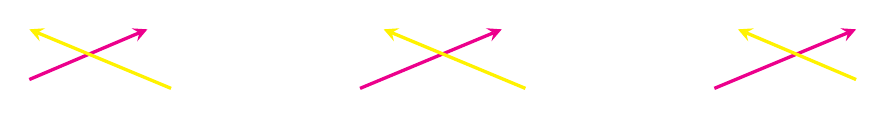
\begin{tikzpicture}[x=1.5mm, y=1.5mm]
        \draw[-stealth,very thick,magenta](-20,-4.25) -- (-10,0);
        \draw[stealth-,very thick,yellow](-20,0) -- (-8,-5);
        \dllnode{0}{0}{0}
        \draw[-stealth,very thick,magenta](8,-5) -- (20,0);
        \draw[stealth-,very thick,yellow](10,0) -- (22,-5);
        \dllnode{30}{0}{0}
        \draw[-stealth,very thick,magenta](38,-5) -- (50,0);
        \draw[stealth-,very thick,yellow](40,0) -- (50,-4.25);
    \end{tikzpicture}
    \caption{Nodes in a doubly-linked list consist of the payload data and references that point to the previous and next nodes.}\label{fig:doubly-linked-list}
\end{figure}

Inserting new node, $C$ between adjacent nodes $A$ and $B$ (where $B = A.next$ and $A = B.previous$) requires connecting $C.previous$ to $A$ and $C.next$ to $B$, and re-assigning $A.next$ to $C$ and $B.previous$ to $C$.

Modify your \function{insert_after()} function to update not only the \lstinline{next} pointers but also the \lstinline{previous} pointers so that \lstinline{new_node} is placed between \lstinline{existing_node} and the node that originally was located immediately after \lstinline{existing_node}.
Modify your \function{insert_after()} and \function{respond()} functions to take advantage of the \lstinline{previous} pointers.

After the program compiles without warnings or errors, you may want to use \function{print_list} to confirm that the \lstinline{previous} pointers are updated correctly.
If your program requires more than a few seconds to build the list, there is a bug in your code.

Creating a circular doubly-linked list is worth another point.
This would be a good time to make a backup copy of your code or to commit it to a private Git repository.

\subsubsection{Inserting Words, Revisited: Working with Unsorted Files} \label{subsubsec:insertionsort}

In Section~\ref{subsec:inserting-words}, you had the option of simplifying your code by treating the last word added as the head of the list instead of traversing the list to find the correct location for a word.
To work with unsorted files, you will need a way to build and maintain a sorted list -- the insertion sort algorithm is a good choice.
You might also want to modify your code to create a circular doubly-linked list.

\paragraph{Insertion Sort}

While you probably learned about sorting in \cstwo, you may not have learned about \textit{Insertion Sort}.
If you did learn about Insertion Sort, you probably learned that it's a $\mathcal{O}(n^2)$ algorithm that is less efficient than $\mathcal{O}(n \log n)$ sorting algorithms such as Merge Sort and Quick Sort.
Insertion Sort has a particular advantage in that it can be applied \textit{as the list is built}, making for a much simpler and less error-prone implementation than a different sort that requires the list to already be built.

The Insertion Sort algorithm reads an input and then traverses a sorted list to find the proper location in the sorted list for the input.
The input is then inserted into the list at that location.

Your current implementation of \function{insert_word()} might be based off of the assumption that the word is either another instance of the last word to be added to the list or is not present in the list.
Update \function{insert_word()} so that it looks for the word in the sorted list.
If the word is found in its proper location in the sorted list, then update the number of occurrences as before.
If the word is not present in its proper location in the sorted list, then insert a new node for that word at its proper location in the sorted list.
If your program requires more than a few seconds to build the list, there is a bug in your code.

Building a list of up to 200 words and generating the correct response when the ``book'' file is unsorted is worth two points (regardless of whether the list is singly- or doubly-linked).
This would be a good time to make a backup copy of your code or to commit it to a private Git repository.

\subsubsection{Inserting Words Revisited: Working with Large Files}

Your code might already be able to handle large files in just a few seconds, in which case you are finished.

On the other hand, your code might run briskly when working with smaller files of only a couple of hundred words but then become very sluggish when the number of words is in the thousands.
This tends to be due to one (or both) of two causes.
Look for inefficient algorithms, and look for memory leaks.
If you use the \texttt{top} utility while running your program, and you notice that your program is allocating more than 10MB, then you probably have a memory leak.
If your program is allocating more than 1GB, then your program most certainly has a memory leak.

Being able to generate a list from a file of up to 80,000 pre-sorted words and generating the correct response, all within 20 seconds, is worth two points.
Being able to do so from a file of up to 80,000 unsorted words is worth another point.
